\documentclass[11pt]{beamer}
\usepackage{beamerthemesplit}
\usepackage{lmodern}
%\usepackage[english,spanish]{babel}
\usepackage[latin1]{inputenc} 
\usepackage{amsmath,amsfonts,amssymb}
\usepackage{subfigure}
\usepackage{rotating}
\usepackage{color,url,natbib}
\usepackage{algorithmic}
\usepackage{algorithm}
\usepackage{comment}
\usepackage{booktabs}
\usepackage{multirow}

\usetheme{CambridgeUS}
%\usetheme{Darmstadt}
%\usetheme{Warsaw}
%\usecolortheme{beaver}
%\usefonttheme{structurebold}
%\usepackage{pgf,pgfarrows,pgfnodes,pgfautomata,pgfheaps}
\usepackage{amsmath,amssymb}
\usepackage{bm}
\usepackage{verbatim}
\usepackage{graphicx}
\usepackage[active]{srcltx}
\usepackage{comment}
\usepackage{color, colortbl}
\setbeamercolor{structure}{fg=blue!70!black!}% to modify  immediately all palettes
\definecolor{Gray}{gray}{0.9}
\definecolor{LightCyan}{rgb}{0.3,0.8,1}
\definecolor{LightCyan}{rgb}{1,.5,1}



\usepackage[first=0,last=9]{lcg}
\newcommand{\ra}{\rand0.\arabic{rand}}



\newcolumntype{g}{>{\columncolor{LightCyan}}c}

 %\usepackage[footnotesize]{caption} 
\usepackage[font=scriptsize,labelfont=scriptsize]{caption}
%\setbeamercovered{dynamic}
%\usepackage{bbding}
\setbeamertemplate{navigation symbols}{} 

\title[\hspace{2em}\insertframenumber/\inserttotalframenumber]{Gamma and Lognormal kernels with stochastic distance for texture parameter estimation under the intensity multilook $\mathcal G_I^0$ law}
\author[\Tiny{J. Cassetti, A. C. Frery}]{J. Cassetti$^1$, A. C. Frery$^2$}
\institute[\Tiny UNGS$^1$-UFAL$^2$]{$^1$Universidad Nacional de General Sarmiento, Argentina\\$^2$Universidade Federal de Alagoas, Brazil}
\date[Jornadas de Matem�tica y Aplicaciones]{ \\
	Junio 2019}

\AtBeginSection[]{\frame{\frametitle{Organization}\tableofcontents[current]}}

\begin{document}

\frame{\titlepage}

\section[Introduction]{Introduction}

\begin{frame}
	\frametitle{Synthetic Aperture Radar}
	\begin{itemize}
	\item A Synthetic Aperture Radar (SAR) is a remote sensing system that emits its own energy in the microwave frequency range
	and records the return from the target. 
	\item This system processes the information captured by the radar antenna combining the information obtained from several sweeps of the antenna to recreate a single ``virtual sweep''. 
	\item This processing provides the same performance as if it had a much larger antenna than the one it actually has.
	\end{itemize}
	\begin{figure}[ht]  
	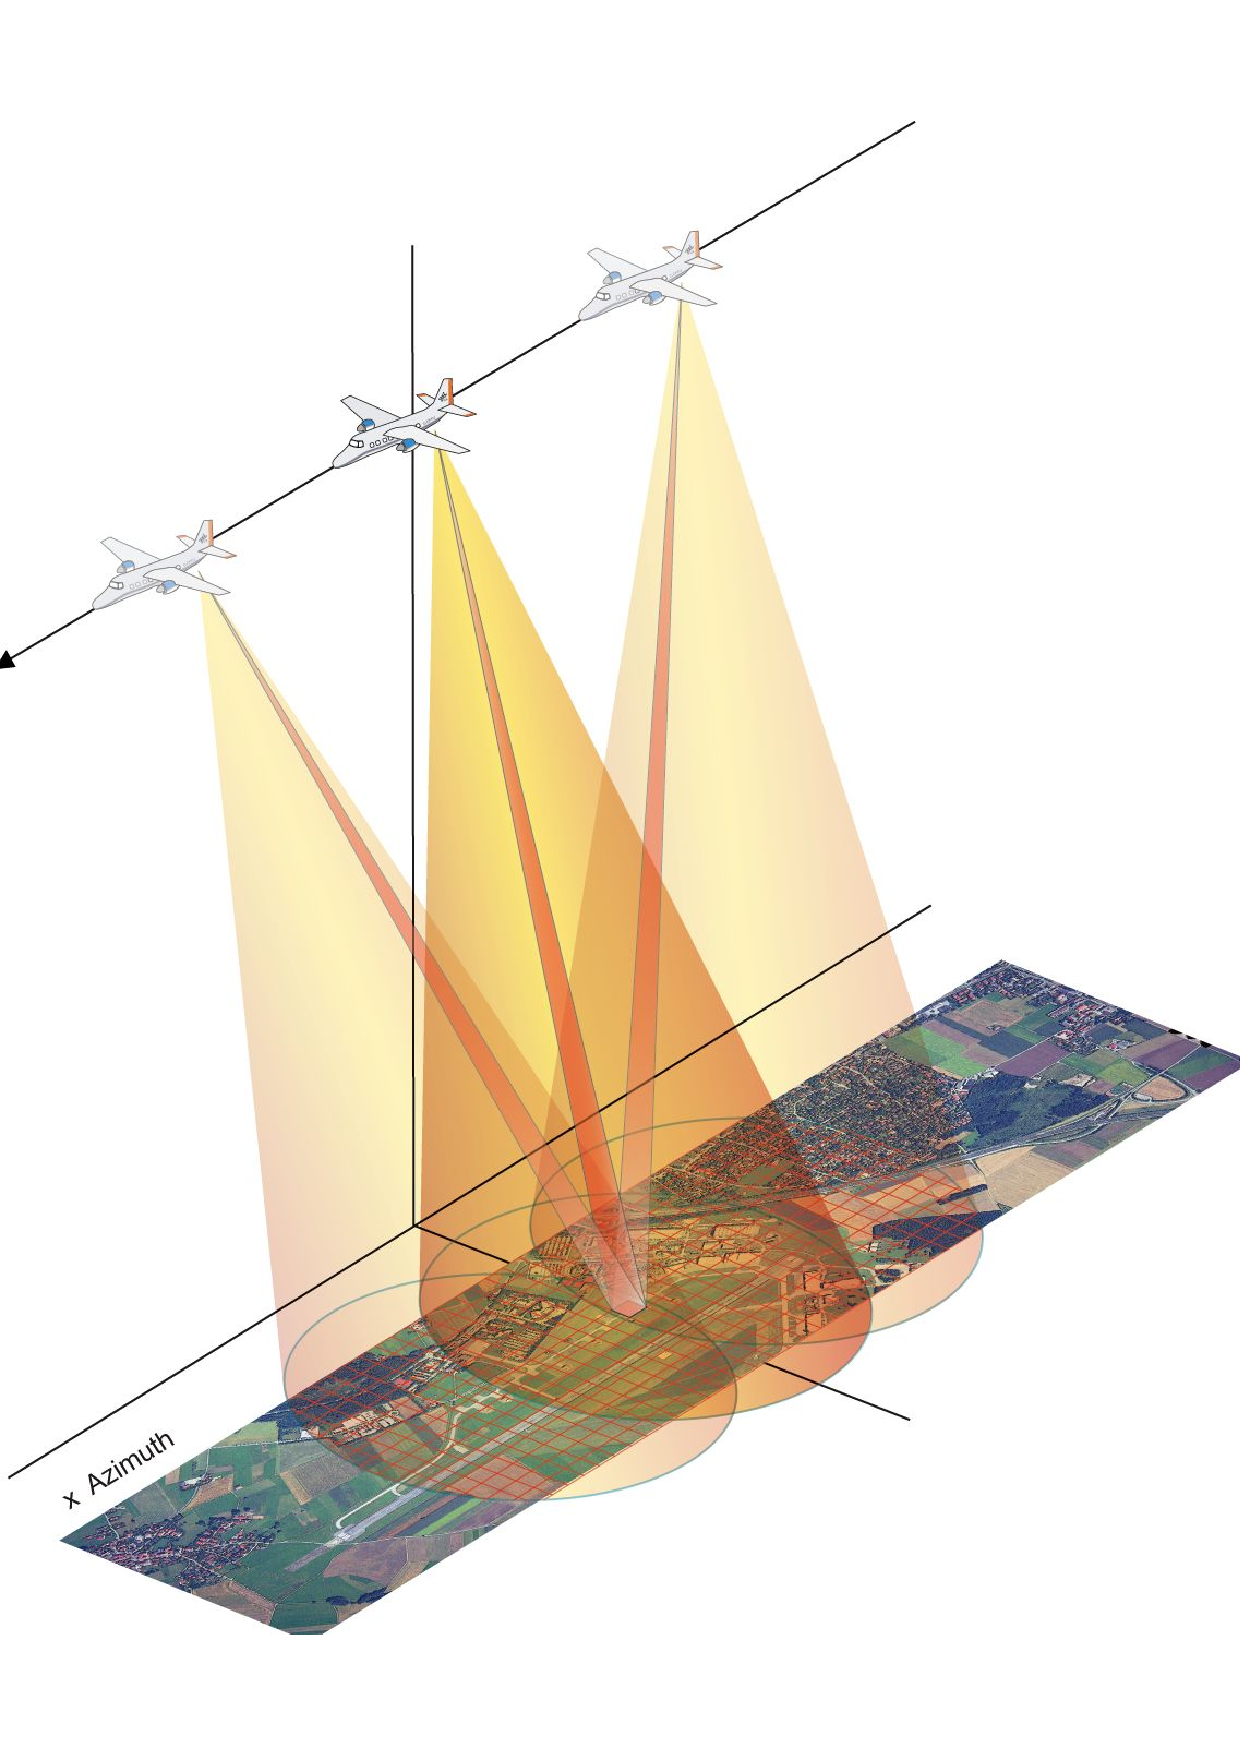
\includegraphics[scale=0.13]{../../../Images/aviao.pdf}
	\end{figure}
\end{frame}

%\begin{frame}
%	\frametitle{Radares SAR en Argentina}
%	\begin{itemize}
%	\item En Argentina se est\'an desarrollando dos radares espaciales SAR para funcionar a bordo de los sat�lites SAOCOM.
%	In Argentina two radars SAR are being developed to function  over the SAOCOM satelites
%	\medskip
%	\item This is a collaborating work between CONAE, CNEA, IAR e INVAP.
%	\item Los sat�lites SAOCOM se encuentran en construcci�n y tienen fecha estimada de puesta en �rbita para fines del a�o 2015 y fines de 2016. 
%	\item Estos sat\'elites fueron dise�ados espec�ficamente para prevenir, monitorear, mitigar y evaluar cat�strofes naturales.
%	\end{itemize}
%\end{frame}

\begin{frame}
	\frametitle{Advantages and disadvantages of SAR images}
	\begin{itemize}
		\item Advantages
		\begin{itemize}
		\item Independence from sunlight%: el radar de im�genes posee un sistema de iluminaci�n propio que permite la adquisici�n tanto de d�a como de noche.
		\medskip
		\item Independence from the weather%: la radiaci\'{o}n electromagn\'{e}tica a las frecuencias de ope\-raci\'{o}n de los sistemas SAR atraviesa las nubes sin atenuaci\'{o}n, por lo tanto el clima no es una limitaci�n en el proceso de adquisici�n de im�genes.
		%\item<3->\textbf{Operaci�n en diferentes polarizaciones}%: la polarizaci�n del radar puede ser horizontal o vertical, esto permite obtener distintos tipos de informaci�n sobre una mismo objetivo.
		\item Provides more information about the texture of the ground.
		\end{itemize}
		\medskip
		\item Disadvantages
		\begin{itemize}
		\item Noisy
		\medskip
		\item Low contrast
		\medskip
		\item Granular appearance
		%\medskip
		%\item Dif�cil An�lisis e Interpretaci�n.
		\end{itemize}
	\end{itemize}
\end{frame}

\begin{frame}
	\frametitle{E-SAR images from the outskirts of the city of Munich, Germany}
	\begin{figure}[ht]
		\centering    
		\subfigure[]{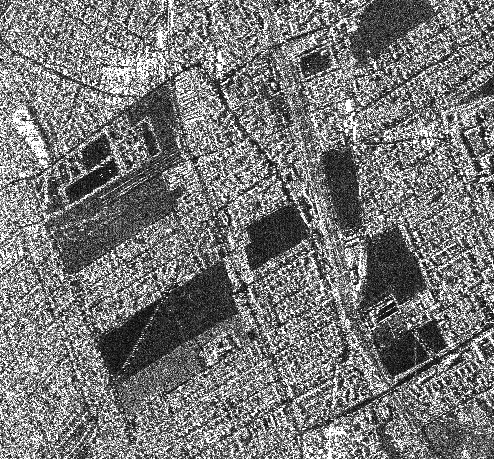
\includegraphics[width=.48\linewidth,height=5cm]{../../../Images/test.png}}
		\subfigure[]{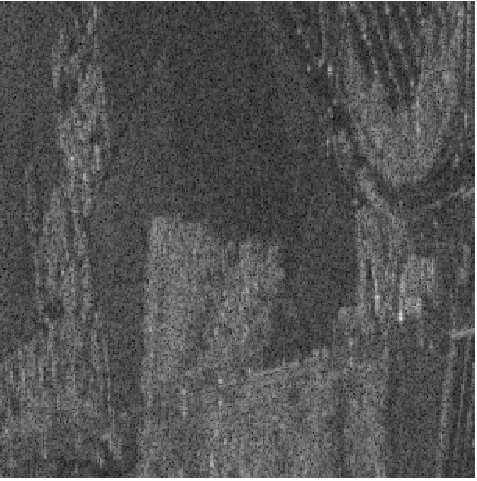
\includegraphics[width=.48\linewidth,height=5cm]{../../../Images/ImHorrible.pdf}}
	\end{figure}
\end{frame}

\begin{frame}
\frametitle{Speckle noise}
\begin{itemize}
\item It is a non-Gaussian noise, and therefore, different from the noise present in optical images.
\bigskip
\item It is present in SAR images because it is inherent to the process of image capture.
\bigskip
\item A technique used to reduce this noise is to generate multiple views or looks of the image during its generation.
%Una t�cnica utilizada para reducir este ruido es generan varias �vistas� o looks de la imgaen durante el proceso de generaci�n de la misma.
\bigskip
\item These looks are averaged generating an image with less noise, but losing resolution.
%Se promedian estos looks generando una imagen multilook con menor ruido speckle pero perdiendo resoluci�n.
\end{itemize}
\end{frame}

%\begin{frame}
%\frametitle{Statistical Model}
%\begin{itemize}
%\item Speckled data have been described under the multiplicative model using the $\mathcal{G}$ family of distributions: $\mathcal G_I^0$ for intensity data.
%\bigskip
%\item This model is able to describe textured and extremely textured areas better than the $\mathcal{K}$ distribution as well as data from textureless areas. 
%\bigskip
%\item Under the $\mathcal G_I^0$ model, regions with different levels of texture can be characterized by the parameters of the distribution.
%\bigskip
%\item Therefore, the accuracy of estimates is very important.
%\bigskip
%%\item Moments and maximum likelihood estimation methods are good for the case of large data samples.
%\bigskip
%\end{itemize}
%\end{frame}

%\begin{frame}
%\frametitle{The proposal}
%\begin{itemize}
%\item Information Theory (IT) provides us with a notion of distance between densities.
%\medskip
%\item We use these notion of distance to propose an estimator of the parameter distribution.
%\medskip
%\item In a previous work we assessed the Hellinger, Bhattacharyya, R�nyi and Triangular distances. 
%\medskip
%\item We concluded that the latter outperforms the others in a variety of situations.
%\bigskip
%%\item Asymmetric kernel are good estimator for density functions with bounded support. Stochastic distance with asymmetric kernel estimator of the underlying density function, provides good estimator of the textured parameter of the $\mathcal G_I^0$ distribution. 
%\end{itemize}
%\end{frame}

\section[The model]{The $\mathcal{G}_I^0$ Model}

\begin{frame}
\frametitle{The Multiplicative Model}
The return in monopolarized SAR images can be modeled
as the product of two independent random variables.
\begin{equation*}
Z=X \cdot Y  
\end{equation*}
where $Z$ represents the return in each pixel, $X$ corresponds to the backscatter, and $Y$ to the
speckle noise. \\ 
\bigskip
For intensity data,  we assume that:\\
$Y \sim \Gamma ( L,L) $, where $L$ is the number of looks, and that \\
$X \sim \Gamma ^{-1}( \alpha ,\gamma ) $, \\
then the return $Z \sim \mathcal{G}_I^{0}( \alpha ,\gamma, L )$.
\end{frame}

\begin{frame}
\frametitle{Density}
The model is specified by the density
\begin{equation*}
f_{\mathcal{G}_I^{0}}( z) =\frac{L^{L}\Gamma ( L-\alpha
) }{\gamma ^{\alpha }\Gamma ( -\alpha ) \Gamma (
L) }\cdot  
\frac{z^{L-1}}{( \gamma +zL) ^{L-\alpha }},
\label{ec_dens_gI0}
\end{equation*}
where $-\alpha,\gamma ,z>0$ and $L\geq 1$ are the texture, the scale and the number of looks.
\bigskip
The $r$th order moments are given by
\begin{equation*}
E(Z^r) =\Big(\frac{\gamma}{L}\Big)^r\frac{\Gamma ( -\alpha-r )}{ \Gamma (-\alpha) }\cdot  
\frac{\Gamma (L+r )}{\Gamma (L)} .
\label{moments_gI0}
\end{equation*}
This moments are finite if $-\alpha > r$.
\end{frame}

\begin{frame}
\frametitle{Parameter Interpretation}
\begin{block}{}
One of the most important features of the $\mathcal{G}_I^0$ distribution is the interpretation of the $\alpha$  parameter, which is related to the texture of the target.  
\end{block}\pause
\begin{table}
\centering
		\begin{tabular}{|c|c|c|c|}
			\hline
      $\alpha$ Value & $(-1,-3]$ & $(-3,-6]$ & $(-6,-\infty)$\\
			\hline
				Texture &Extremely Textured &  Textured & Non Textured\\
				\hline
		\end{tabular}
\end{table}\pause

%\begin{block}{}
%	In the following we employ $\gamma^*$ such that $E(Z)=1$.  This condition gives a relation %between $\gamma \text{ and } \alpha: \, \gamma^* =-\alpha-1$
%\end{block}

\begin{block}{Purpose}
	In the following we employ $\gamma^*$ such that $E(Z)=1$, to make the results comparable:  
	$$\gamma^* =-\alpha-1.$$ 
\end{block}
\end{frame}

\begin{frame}
	\frametitle{Parameter Estimation}
	\begin{itemize}
		\item Parametric estimator: Maximum Likelihood Estimator.
		\begin{align*}
			\widehat{\alpha}_{{\text{\tiny{MV}}}}=\arg\max_{\alpha} \log(L(\alpha)/\vec{Z}=\vec{z}).
		\end{align*}
		\begin{align}
		%%% ACF Revisala, la segunda l�nea est� rara
			\nonumber \log(L(\alpha)/\vec{Z}=\vec{z})&=n(L \log(L)+\log[\Gamma(L-\alpha)]-\log(\Gamma(L))\\
			\nonumber&-\log(\Gamma(-\alpha))-\alpha \log(-\alpha-1)) + (L-1) \sum_{i=1}^n \log(z_i))\\
			\nonumber&-(L-\alpha) \sum_{i=1}^n \log(-\alpha-1+z_i L).
		\end{align}
	\end{itemize}
\end{frame}

\begin{frame}
	\frametitle{Parameter Estimation}
	\begin{itemize}
	\item Non Parametric Estimator: Minimizing Stochastic Distances between the theoretical density function and a nonparametric estimator of the underlying density function.
	\medskip
	\begin{equation*}
	\widehat\alpha= \arg\min_{\alpha} d\big(f_{\mathcal{G}_I^{0}}(\alpha,\gamma^*, L ), \widehat{f}(\textbf{z})\big)
	\label{minimization}
	\end{equation*}
	\end{itemize}
\end{frame}
%\section[MLE]{Maximum Likelihood Estimator}
%
%\begin{frame}
%\frametitle{Maximum Likelihood Estimator}
%
%The Maximum Likelihood Estimator (ML) of the texture parameter, assuming $\gamma^*=-\alpha-1$ and $L$ known, is:
%\begin{align*}
%	\widehat{\alpha}_{{\text{\tiny{MV}}}}=\arg\max_{\alpha} \log(L(\alpha)/\vec{Z}=\vec{z}).
%\end{align*}
%\begin{align}
%	\nonumber \log(L(\alpha)/\vec{Z}=\vec{z})&=n(L \log(L)+log(\Gamma(L-\alpha))-\log(\Gamma(L))\\
%	\nonumber&-\log(\Gamma(-\alpha))-\alpha \log(-\alpha-1)) + (L-1) \sum_{i=1}^n \log(z_i))\\
%	\nonumber&-(L-\alpha) \sum_{i=1}^n(\log(-\alpha-1+z_i L))).
%\end{align}
%\end{frame}
%
%\begin{frame}
%\frametitle{ Using $\gamma^*=-\alpha-1$}
%\begin{itemize}
%	\item The ML estimator of $\alpha$, $\widehat\alpha_{\text{ML}}$,  based on $\textbf{z}$, is the solution of the following nonlinear equation
%	\begin{eqnarray*}
%	\small
%	&\psi^0(\widehat{\alpha}_{\text{ML}})-\psi^0(L-\widehat{\alpha}_{\text{ML}})-\log(1-\widehat{\alpha}_{\text{ML}})+
%	\dfrac{\widehat{\alpha}_{\text{ML}}}{1-\widehat{\alpha}_{\text{ML}}}+\\
%	&\dfrac{1}{n}\sum_{i=1}^n{\log(1-\widehat{\alpha}_{\text{ML}}+Lz_i)}- 
%	\dfrac{\widehat{\alpha}_{\text{ML}}-L}{n}\sum_{i	=1}^n \dfrac1{1-\widehat{\alpha}_{\text{ML}}+Lz_i}= 0 
%	\label{derloglikelihood_gI0}
%	\end{eqnarray*}
%	where $\psi^0(\cdot)$ is the digamma function.
%	\bigskip
%	\bigskip
%	\item No explicit solution for this system is available in general.
%	\medskip
%	\item Therefore, numerical routines are required.  We used the BFGS optimization algorithm.
%\end{itemize} 
%\end{frame}
%
%\begin{frame}
%	\frametitle{Maximum Likelihood Estimator}
%\begin{figure}[hbt]
%	\centering    
%	\label{MV}
%	\subfigure[$\alpha=-1.5$]{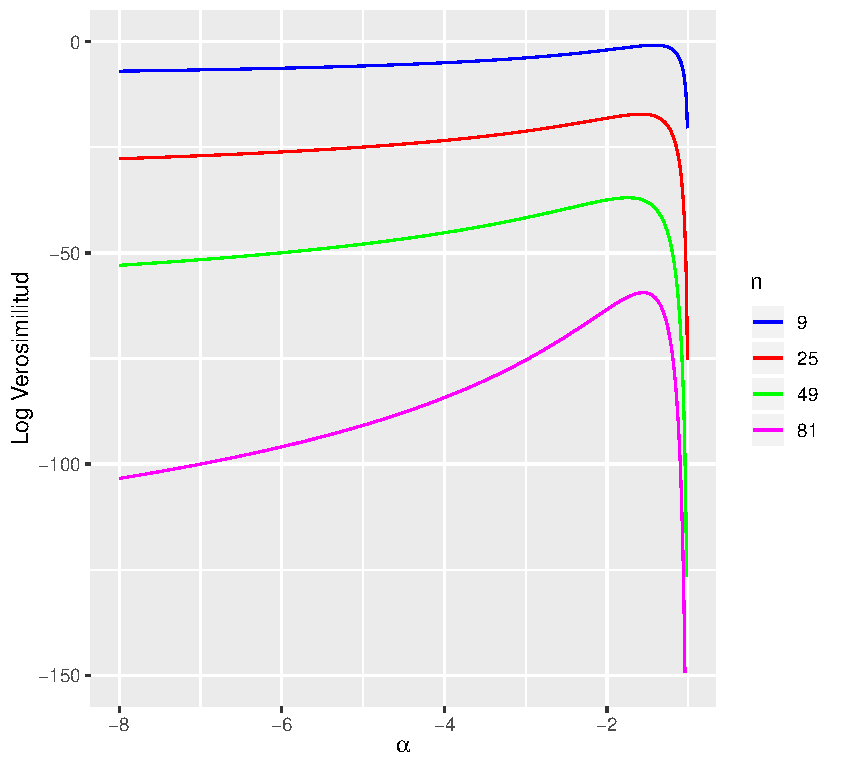
\includegraphics[scale=0.4]{../../../Figures/Tesis/Capitulo4/Verosimilitud1punto5_2.pdf}}
%	\subfigure[$\alpha=-5$]{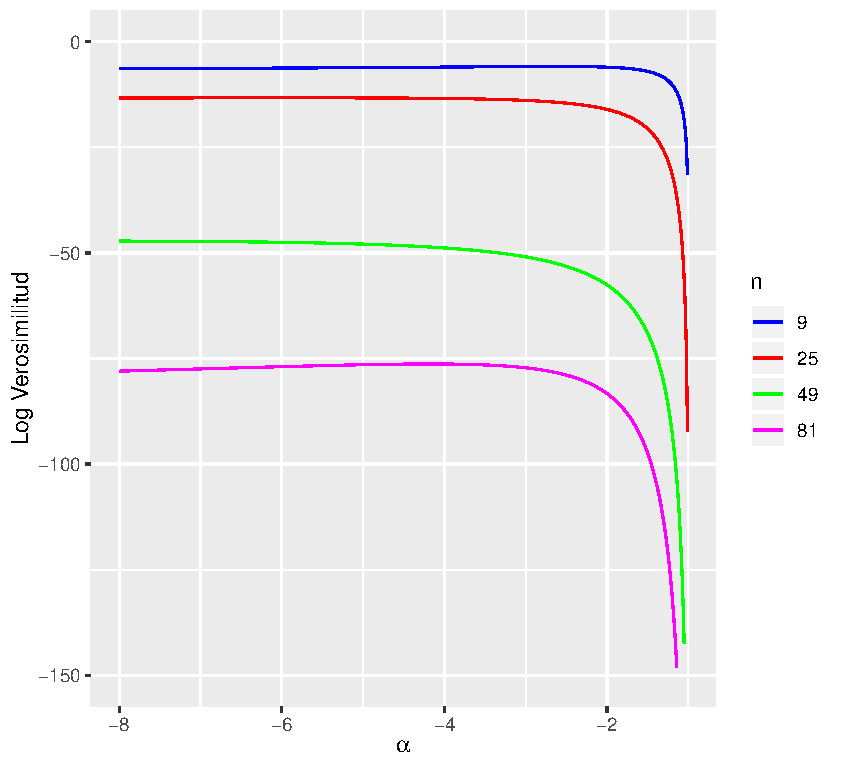
\includegraphics[scale=0.4]{../../../Figures/Tesis/Capitulo4/Verosimilitud-5_2.pdf}}
%	\caption{Log Liklihood for $L=3$}
%\end{figure}
%\end{frame}

\section[Stochastic Distances]{Stochastic Distances}

\begin{frame}
\frametitle{Stochastic Distances}
\begin{itemize}
\item Stochastic Distances allow the comparison between two density functions. 
\medskip
\item We studied several distances and chose\dots
\item Triangular Distance\\
\medskip
Let $V$ and $W$ be two random variables defined over the same probability space whose density functions are $f_V(x;\theta_1)$ and $f_W(x;\theta_2)$, respectively.
The Triangular distance is defined as:
\medskip
$$d_T(f_V,f_W)=\int_{-\infty}^{\infty}\frac{(f_V-f_W)^2}{f_V+f_W}dx.$$

\end{itemize}
\end{frame}


\begin{frame}
	\frametitle{Choosing distances}
	\begin{block}{}
		We conducted a Monte Carlo experiment with 500 replications for several parameter values; for each case $\{\widehat{\alpha}_1, \dots, \widehat{\alpha}_{500}\}$ are obtained by simulation.
	\end{block}
	\bigskip
	\begin{block}{}
		\begin{itemize}
			\item $\alpha\in\{-1.5, -3, -5, -8\}$
			\medskip
			\item Two levels of $L\in\{3,8\}$
			\medskip
			\item  $n\in\{9, 25,49, 81,121,500\}$
			\item Initially estimate $\widehat{f}(z)$ with histograms.
			%%% ACF Yo sacar�a todo lo que se refiere a estimaci�n con histograma
			\item We evaluate the estimators through the bias and the mean squared error.
		\end{itemize}
	\end{block}
	
\end{frame}


%\begin{frame}
%\frametitle{Stochastic Distances}
%Let $V$ and $W$ be two random variables defined over the same probability space whose density functions are $f_V(x;\theta_1)$ and $f_W(x;\theta_2)$, respectively.
%The Triangular distance is defined as:
%\medskip
%$$d_T(V,W)=\int_{-\infty}^{\infty}\frac{(f_V-f_W)^2}{f_V+f_W}dx.$$
%\end{frame}

\begin{frame}
	\frametitle{Distances}
	\begin{itemize}
		\item $\alpha$ estimated for L=3 and different distances.
	\end{itemize}
	\begin{figure}[ht]
		\centering    
		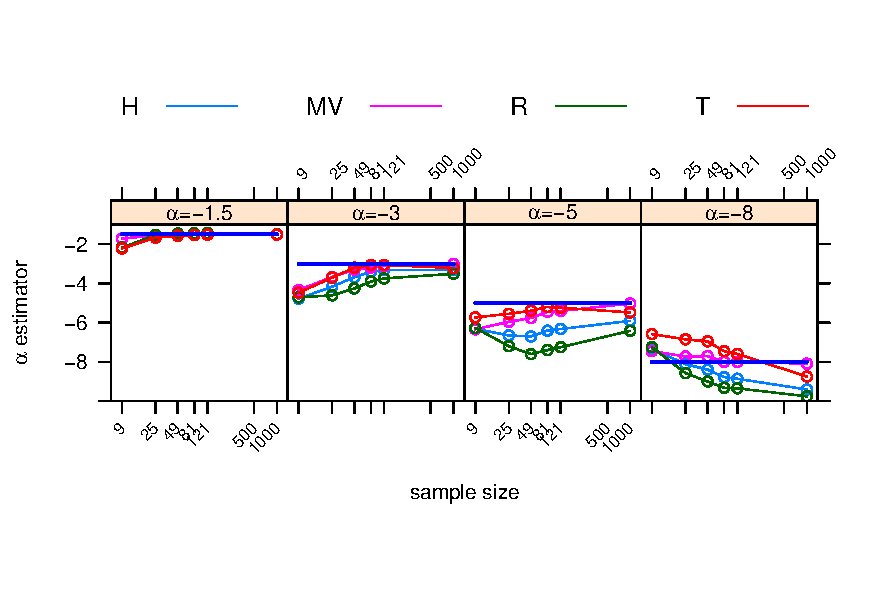
\includegraphics[scale=0.8]{../../../Figures/JornadasDoctorado/alfa_escSemiLog_L3AST.pdf}
	\end{figure}
\end{frame}

\begin{frame}
	\frametitle{Distances}
		\begin{itemize}
		\item MSE estimated for L=3 and different distances.
	\end{itemize}
	\begin{figure}[ht]
		\centering    
		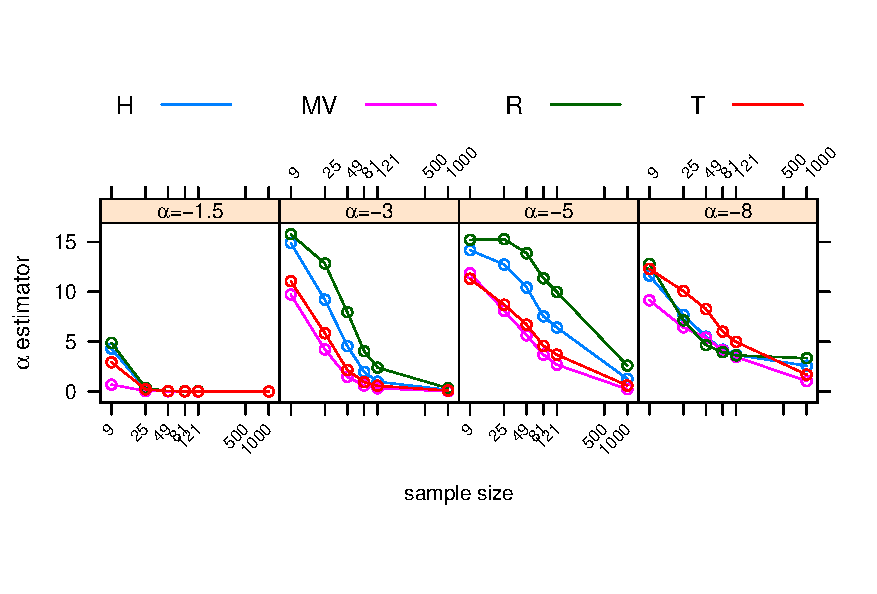
\includegraphics[scale=0.8]{../../../Figures/JornadasDoctorado/ECM_escSemiLog_L3AST.pdf}
	\end{figure}
\end{frame}


%\begin{frame}
%	\frametitle{Published papers}
%	\begin{itemize}
%		\item J. Cassetti, J. Gambini, A. Frery - \emph{``Estimaci�n de Par�metros utilizando Distancias Estoc�sticas para Datos con Ruido Speckle"}, Anales de la 42 JAIIO - 2013 - ISSN 1850-2776.
%		
%		\item J. Cassetti, J. Gambini, A. Frery - \emph{``Parameter Estimation in SAR Imagery using Stochastic Distances"} - The 4th Asia-Pacific Conference on Synthetic Aperture Radar, Tsukuba, Jap�n - pag. 573-576 - 2013- INSPEC Accession Number: 14026655.
%		
%		\item J. Gambini, J. Cassetti, M. Lucini, A. Frery  - \emph{``Parameter Estimation in SAR Imagery using Stochastic Distances and Asymmetric Kernels"} - IEEE Journal of selected topics in appplied earth observations and remote sensing - 8 (1), 365-375 -2014-DOI:10.1109/ JSTARS.2014.2346017.
%	\end{itemize}
%\end{frame}
   
\section[AK]{Asymmetric Kernels}

%\begin{frame}
%\frametitle{Asymmetric Kernels}
%\begin{block}{}
% When the support of the underlying density is unbounded, symmetric kernels have a good performance.
%\end{block}{}
%\medskip
%\begin{block}{}
%Their consistence is well documented.
%\end{block}{}
%\bigskip
%But\ldots
%\bigskip
%\begin{alertblock}{}
% When the support of the underlying density is bounded, standard symmetric kernels lead to boundary bias.
%\end{alertblock}{}
%\medskip
%\begin{alertblock}{}
%Because the standard symmetric kernels assign weight outside the support, when smoothing is carried out near the boundary.
%\end{alertblock}{}
%\end{frame}

\begin{frame}
	\frametitle{Asymmetric Kernels}
	\begin{figure}[ht]
	\centering    
	\includegraphics[scale=0.6]{../../../Figures/JornadasDoctorado/Asymmetrickernel.pdf}
\end{figure}

\end{frame}

\begin{frame}
	\frametitle{Asymmetric Kernels}
	Let $\bm X = (X_1,\dots, X_n)$ be a random sample of size $n$, with an unknown density probability function $f$, the estimating density function using asymmetric kernels is given by 
	$$
	\widehat{f}_b(x)=\frac{1}{n}\sum_{i=1}^n K_{\vec{\theta}(b,x)}(X_i),
	$$ 
	where $b$ is the bandwith of the kernel $K$ and $\vec{\theta}(b)$ is the parameter vector.
\end{frame}

\begin{frame}
	\frametitle{Asymmetric Kernels}
	In this work we assess the following asymmetric kernels: 
	\medskip
	\begin{itemize}
		\item Gamma kernel (NG)
		\begin{align*}
		K_{{\Gamma}_{\vec{\theta}(x,b)}}(t) & =\Gamma_{\left(\frac{x}{b}+1,b\right)}(t)
		\end{align*}
%		\item Reciprocal Inverse Gaussian kernel
%		\begin{align*}
%		K_{{RIG}_{\vec{\theta}(x,b)}}(t) & =RIG_{\left(\frac{1}{x-b},\frac{1}{b}\right)}(t)
%		\end{align*}
		\item Log Normal kernel
		\begin{align*}
		K_{{LN}_{\vec{\theta}(x,b)}}(t) & =LN_{\left(log(x)+b^2,b^2\right)}(t)
		\end{align*}
		for every $t>0$ respectively.
		\item Inverse Gaussian kernel
		\begin{align*}
		K_{{IG}_{\vec{\theta}(x,b)}}(t) & =IG_{(x,\frac{1}{b})}(t)
		\end{align*}
		
		\item We also evaluated differents bandwidth
	\end{itemize}
\end{frame}

%\section[Methodology]{Methodology}
%
%
%\begin{frame}
%	\frametitle{Methodology}
%	\begin{itemize}
%		\item $\textbf{z}=(z_1,\dots, z_n)$ be an independent sample of size $n$ from the $\mathcal{G}_I^{0}(\alpha, \gamma^*, L)$ distribution .
%		\item $\widehat{f_k}$ an estimation, using asymmetric kernel $K$, of the underlying density .
%		\medskip
%		\item The estimator we assess is given by
%		\begin{equation*}
%		\widehat\alpha= \arg\min_{-20\leq\alpha \leq -1} d_T\big(f_{\mathcal{G}_I^{0}}(\alpha,\gamma^*, L ), \widehat{f_k}(\textbf{z})\big), \text{ where }
%		\label{minimization}
%		\end{equation*}
%		\item[] $d_T$  represents the Triangular distance.
%		%\item $\widehat{f_k}$ indicates the estimation of the underlying density function, using each of the kernels assessed. 
%%		\item Let $X_1 \text{ and } X_2$ be random variables, $X_i \sim  \mathcal{G}_I^{0}(\alpha_i,\gamma_i,L)$,  such as $E(X_1)=E(X_2)$ and $\alpha_2=\alpha_1-\Delta, \ \Delta>0, \ d_T(f_{X_1},f_{X_2}) 
%%		\mathop{\longrightarrow }\limits_{\alpha\to -\infty} 0$
%	\end{itemize} 
%\end{frame}
%
%
%\begin{frame}
%\frametitle{Methodology}
%\begin{itemize}
%\item In this case we evaluated different asymmetric kernels such as:
%	\begin{enumerate}[a)]
%	\item Inverse Gaussian
%	\medskip
%	\item Gamma
%	\medskip
%%	\item First kind of Gamma kernel
%%	\medskip
%	\item Log Normal kernel
%	\end{enumerate}
%\bigskip
%\item We also evaluated differents bandwidth
%%	\begin{enumerate}[i)]
%%		\item From $a) \text{ to } c)$ we use the $b_{opt}$ bandwidth.
%%		\medskip
%%		\item For $\Gamma$ kernel we use:
%%		\begin{itemize}
%%		 \item $b_{1}=\frac{1}{5 \sqrt{n}}$
%%		 \medskip
%%		 \item $b_{2}=b_{RIG}$ optimum.
%%		 \end{itemize}
%%		\medskip
%%		\item For $c) \text{ and } d)$ we use the $b_{LSCV}$ bandwidth.
%%	\end{enumerate}
%\end{itemize}
%\end{frame}



\section{Results}

\begin{frame}
\frametitle{Experimental Results}
\begin{block}{}
	We conducted a Monte Carlo experiment with 500 replications for several parameter values; for each case $\{\widehat{\alpha}_1, \dots, \widehat{\alpha}_{500}\}$ are obtained by simulation.
\end{block}

\begin{block}{}
\begin{itemize}
	\item $\alpha\in\{-1.5, -3, -5, -8\}$
	%\medskip
	\item Two levels of $L\in\{3,8\}$
	%\medskip
	\item  $n\in\{9, 25,49, 81,121,500\}$
	\item
	\begin{equation*}
	\widehat\alpha= \arg\min_{-20\leq\alpha \leq -1} d_T\big(f_{\mathcal{G}_I^{0}}(\alpha,\gamma^*, L ), \widehat{f_k}(\textbf{z})\big), 
	\end{equation*}
	\end{itemize}
\end{block}

\begin{block}{}
In order to assess the proposed estimation method, we evaluate
\begin{itemize}
	\item the number of cases of convergence
	%\medskip
	\item computational cost, bias and mean squared error
\end{itemize} 
\end{block}
\end{frame}

%%%%%%%%%%%%%%%%%%%%%%%%%%%%%%%%%%%%%%%%%%%%%%
\begin{comment}
\begin{frame}
\frametitle{Estimators}
\begin{block}{The mean}
 $$
\widehat{E}(\widehat{\alpha}) = \overline{\widehat{\alpha}}=\frac{1}{500}{\sum_{i=1}^{500}{\widehat{\alpha}_i}}
 $$
\end{block}\pause
\begin{block}{The Bias}
  $$\widehat{B}(\widehat\alpha) = \overline{\widehat\alpha}- \alpha$$
\end{block}\pause
\begin{block}{The Mean Square Error}
$$\widehat{\operatorname{mse}}(\widehat\alpha)=\frac{1}{500}{\sum_{i=1}^{500}{(\widehat{\alpha}_i-\alpha)^2}}$$
\end{block}
\end{frame}
\end{comment}
%%%%%%%%%%%%%%%%%%%%%%%%%%%%%%%%%%%%%%%%%%%%%%%%%%%%%%%%

%\begin{frame}
%\begin{block}{}
%\begin{center}
%Without contamination
%\end{center}
%\end{block}
%\end{frame}

\begin{frame}
\frametitle{Number of cases of non-convergence for L=$3$}
\begin{table}[hbt]
	\caption{Number of cases of non-convergence for L=$3$}
	\centering
	\label{MLyLNyNGyIGyLC_L=3}
	\tiny{
		\begin{tabular}{c*6{r}}
			\toprule		
			$\alpha$ & $n$ & $\widehat{\alpha}_{\text{ML}}$ & $\widehat{\alpha}_{\text{NG}}$
			& $\widehat{\alpha}_{\text{LN}}$
			& $\widehat{\alpha}_{\text{IG}}$\\
			\midrule
			\multirow{1 }{*}{$-1.5$} 
			&   $9$ & $0$ & $2$ & $2$ & $1$\\
			&  $25$ & $0$ & $0$ & $0$ & $0$\\
			\midrule
			\multirow{3 }{*}{$-3$} 
			&   $9$ & $57$  & $25$ & $37$ & $\textbf{35}$\\ 
			&  $25$ & $6$   & $2$  & $3$  & $4$\\
			&  $49$ & $1$   & $1$  & $0$  & $0$\\ 
			&  $81$ & $0$   & $0$  & $0$  & $0$\\ 
			& $121$ & $0$   & $0$  & $0$  & $0$\\ 
			\midrule
			\multirow{5 }{*}{$-5$} 
			&   $9$ & $120$ & $51$ & $56$ & $\textbf{79}$\\ 
			&  $25$ & $58$  & $19$ & $23$ & $11$\\ 
			&  $49$ & $21$  & $6$  & $5$  & $5$\\ 
			&  $81$ & $7$   & $2$  & $3$  & $1$\\ 
			& $121$ & $2$   & $0$  & $0$  & $0$\\ 
			& $500$ & $0$   & $0$  & $1$  & $0$\\ 
			\midrule
			\multirow{6 }{*}{$-8$} 
			&   $9$  & $200$ & $79$ & $87$ & $\textbf{117}$\\ 
			&  $25$  & $128$ & $48$ & $56$ & $50$\\ 
			&  $49$  & $86$  & $27$ & $39$ & $22$\\ 
			&  $81$  & $42$  & $19$ & $17$ & $14$\\ 
			& $121$  & $33$  & $9$  & $9$  & $4$\\ 
			& $500$  & $0$   & $0$  & $1$  & $0$\\
			& $1000$ & $0$   & $0$  & $0$  & $0$\\ 
			\midrule
			\bottomrule 	
		\end{tabular}
	}
\end{table}	
\end{frame}

\begin{frame}
	\frametitle{Mean $\widehat{\alpha}$, $L=3$.}
	\begin{figure}[ht]
		\centering    
		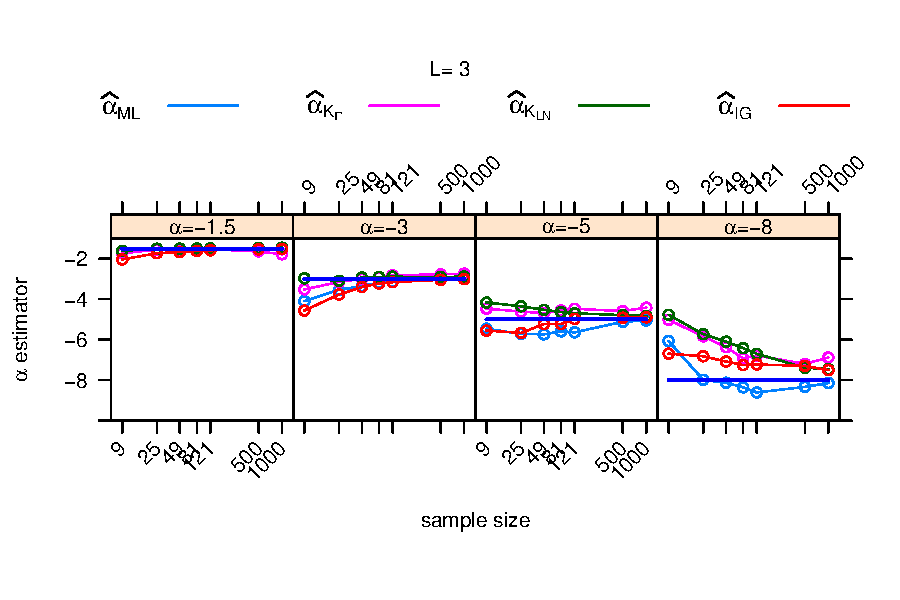
\includegraphics[scale=0.6]{../../../Figures/JornadasDoctorado/alfa500_sinmenos20_MVyLNyNG1yIGJIAIIS_L3.pdf}
	\end{figure}
\end{frame}

\begin{frame}
	\frametitle{MSE $\widehat{\alpha}$, $L=3$.}
	\begin{figure}[ht]
		\centering    
		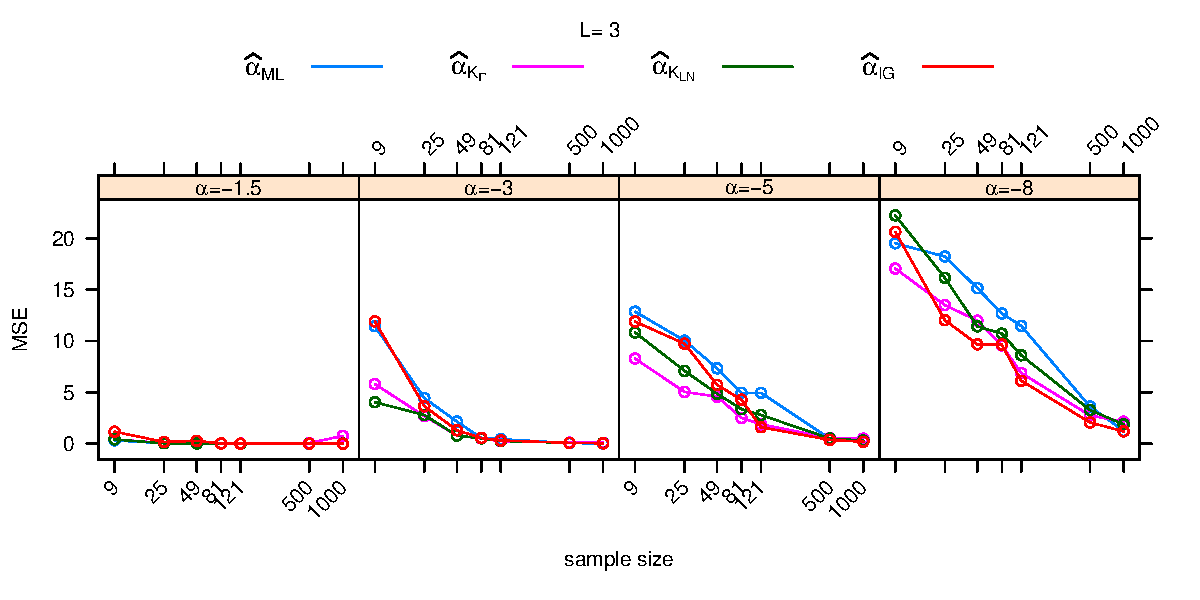
\includegraphics[scale=0.6]{../../../Figures/JornadasDoctorado/ECMa500_sinmenos20_MVyLNyNG1yIGJIAIIS_L3.pdf}
	\end{figure}
\end{frame}


\begin{frame}
	\frametitle{Robustez}
	We  evaluate the robustness of the proposed estimator defining $Z=(1-B)W+BU$ where: $W \sim \mathcal{G}_I^0(\alpha,\gamma^*,L)$ is the true model, $U \sim \mathcal{G}_I^0(\alpha_1,\gamma_1^*,L)$ where $\alpha_1=-15$ and $\gamma_1^*=-\alpha_1-1$, $B \sim Ber(\epsilon)$ where $\epsilon=0.05$. 
	%The cumulative distribution function of $Z$ is $(1-\epsilon) {F}_{\alpha,\gamma^*,L}(z)+\epsilon {F}_{\alpha_1,\gamma_1^*,L}(z)$.
	\begin{figure}[ht]
		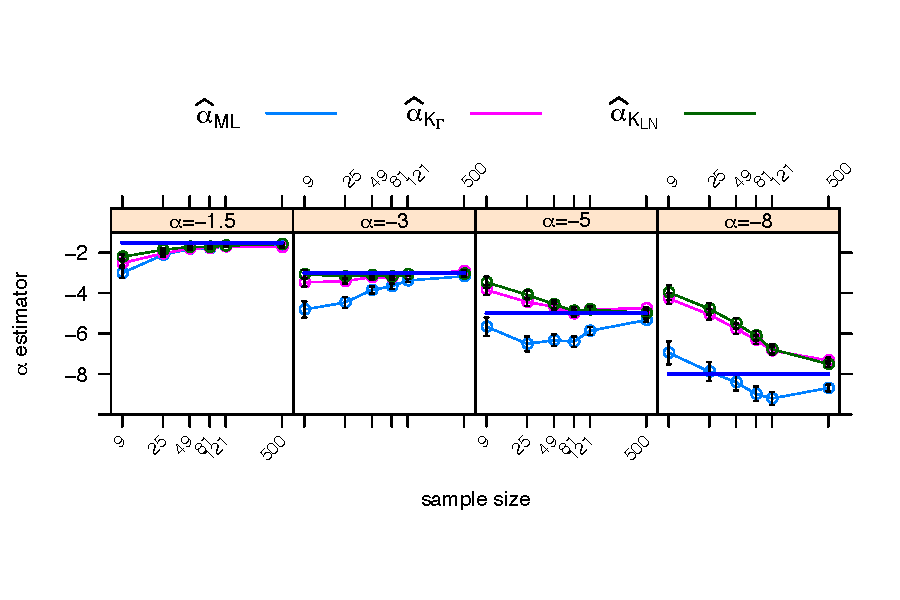
\includegraphics[scale=0.6]{../../../Figures/JornadasDoctorado/alfa500sinmenos20CONTMVconX0yGAyLNOPTIMhasta500MOM1_2_SinCte_Ver2FINAL_L3.pdf}\\
		\caption{\small{Mean value of $\widehat{\alpha}$, $L=3$.}}
	\end{figure}
\end{frame}

\begin{frame}
	\frametitle{Robustez}
		\begin{figure}[ht]
		%	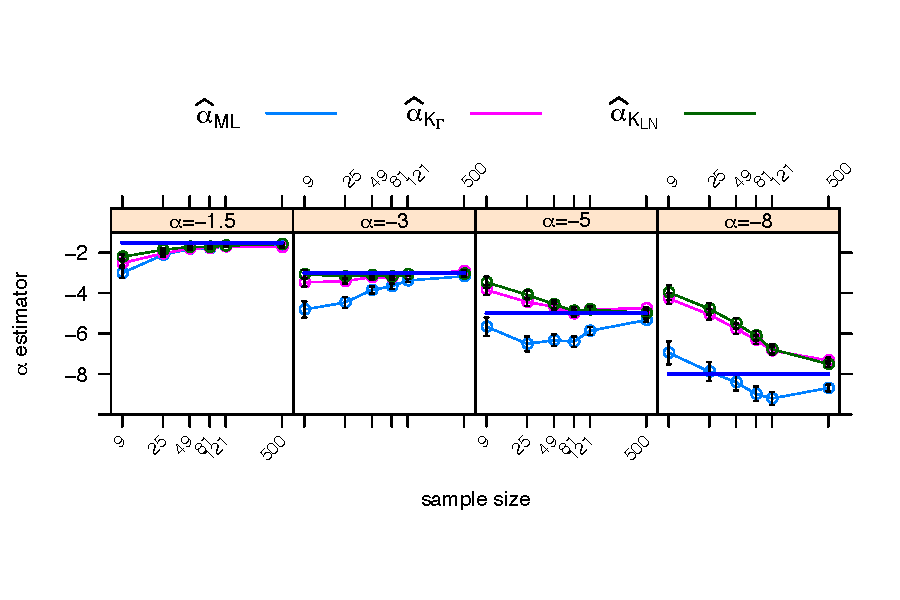
\includegraphics[scale=0.6]{../../../Figures/JornadasDoctorado/alfa500sinmenos20CONTMVconX0yGAyLNOPTIMhasta500MOM1_2_SinCte_Ver2FINAL_L3.pdf}\\
		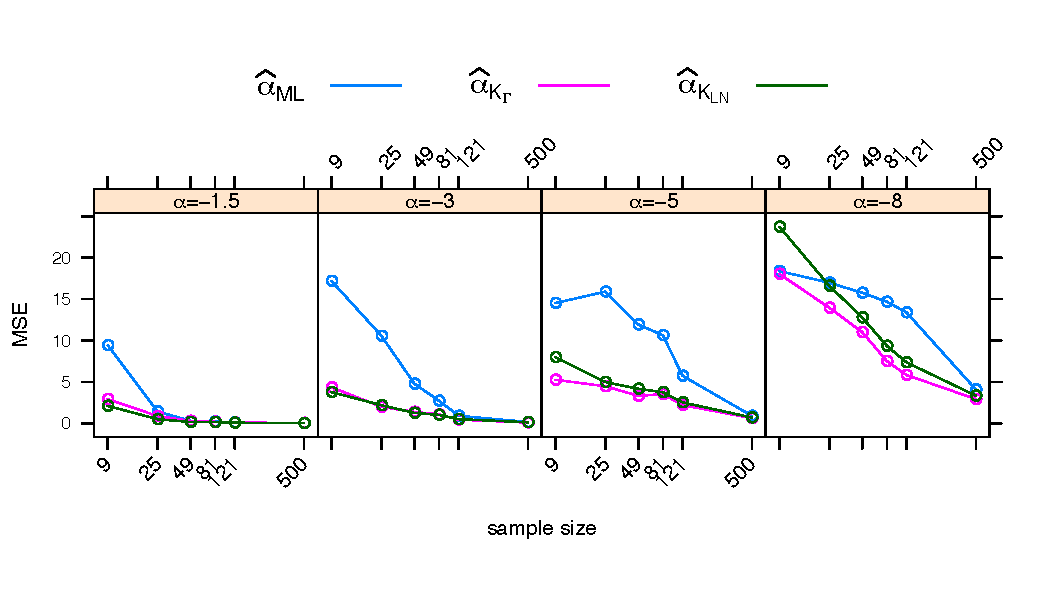
\includegraphics[scale=0.6]{../../../Figures/JornadasDoctorado/ECM_500_L3MVconX0yGAyLN_OPTIM_hasta500_MOM1_2_SinCte_Ver2FINALeps05.pdf}\\
		\caption{\small{Mean squared error of $\widehat{\alpha}$, $L=3$.}}
		\end{figure}
\end{frame}

\begin{frame}
	\frametitle{Stylized Samples}

	The Empirical Influence Function shows the performance of the estimator $\widehat{\alpha}_{\text{\tiny{T}}}$ when $n-1$ observations are fixed, and one ranges over the support of the distribution. It depends on the particular sample so we use the $i^{th}$ quantile of the assumed distribution to characterize the typical observations.
	
	\begin{figure}
		\centering
		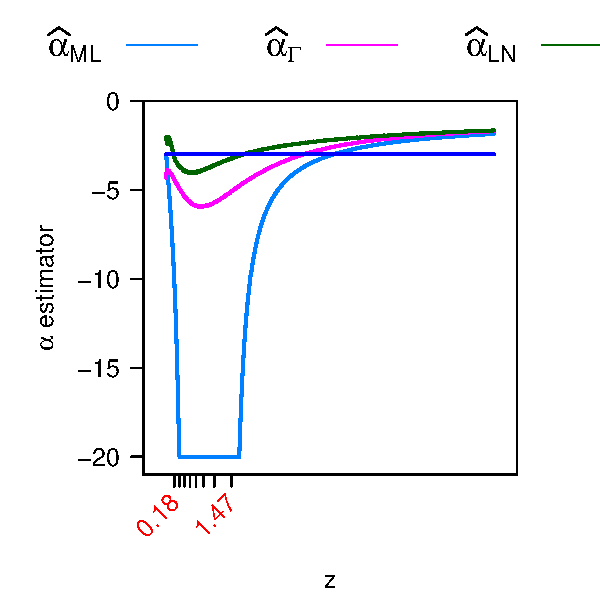
\includegraphics[scale=0.5]{../../../Figures/IVJIAAIS2017/Cont/INFL_LNyMVyGA_alfa-3_L3n9.pdf}
		\captionof*{figure}{\small{SEIFs for $L=3$, $\alpha=-3$ and $n=9$. \label{figure:SEIFL1}}}
	\end{figure}
\end{frame}

\begin{frame}
	\frametitle{New Results-Another bandwidth}
	\begin{figure}
		\centering
		\subfigure[\tiny Without contamination]{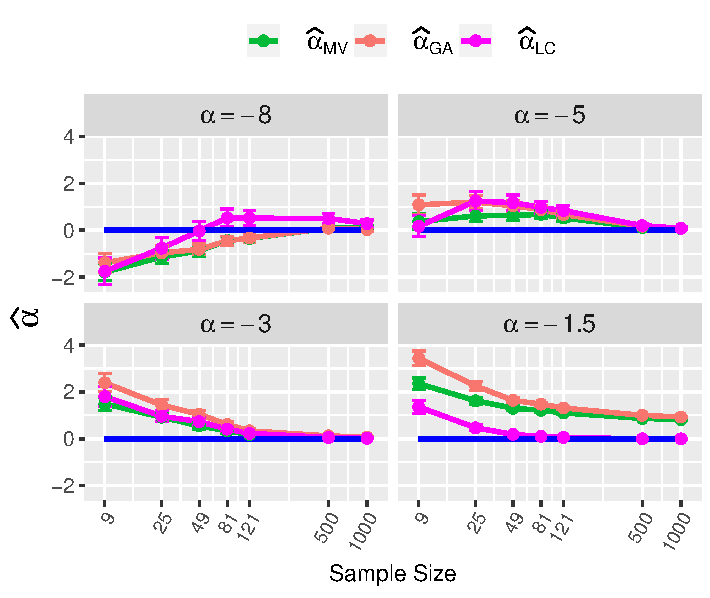
\includegraphics[scale=0.4]{../../../Figures/JornadasDoctorado/SesgoAlfa500Repli_SINCONT_COMUNES_GAyMVyLCygamaEstrBOPTIMO_L3.pdf}}
		\subfigure[\tiny With contamination]{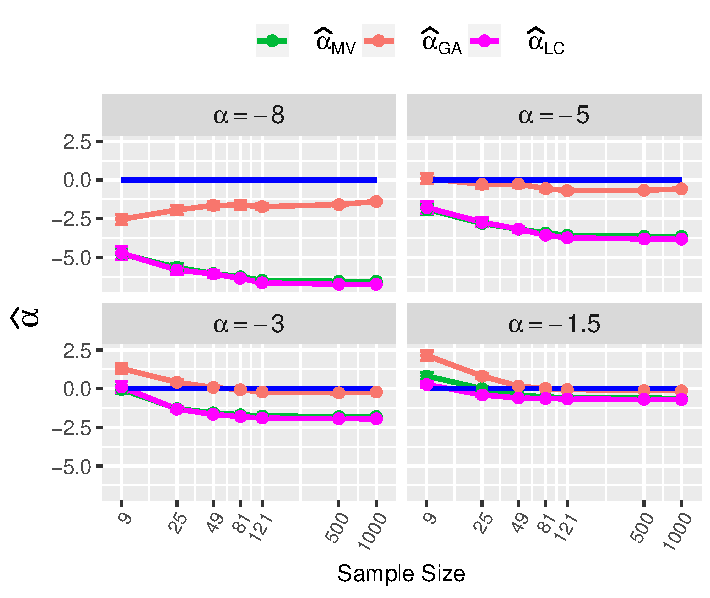
\includegraphics[scale=0.4]{../../../Figures/JornadasDoctorado/SesgoAlfa500Repli_CONT_COMUNES_GAyMVyLCygamaEstrBOPTIMOEps005_L3.pdf}}
		\caption*{}{\small{Bias for $L=3$, $\alpha=-3$. \label{figure:SEIFL1}}}
	\end{figure}
\end{frame}

\begin{frame}
	\frametitle{Theoretical Results}
	\begin{itemize}
		\item 	For all compact interval $[z_{1},z_{2}]\subset{(0,\infty)}$, $f_{\mathcal{G}_I^0}$ converges uniformly to $\Gamma_{(L,1/L)}$ in $[z_{1},z_{2}]$ if $\alpha\to -\infty$, where $\Gamma_{(L,1/L)}$ is the density function of the $\Gamma$ model with parameters ${L,1/L}$.
		\bigskip
		\item 	For all compact interval $[z_{1},z_{2}]\subset{(0,\infty)}$, $f_{\mathcal{G}_I^0}$ converges uniformly to $0$ in $[z_{1},z_{2}]$ when $\alpha\to -1^{-}$.
		\bigskip
		\item Let $\widehat{\alpha}=\arg\min\limits_{\alpha\in [z_{1},z_{2}]} d_{\text{T}}(f_{\mathcal{G}_I^0},\widehat{f})$. Then $\widehat{\alpha}$ is a consistent estimator of $\alpha$, i.e. $\widehat{\alpha}_n \stackrel{p} {\longrightarrow} \alpha$ when $n \rightarrow +\infty$.
	\end{itemize}
\end{frame}

%%%%%%%%%%%%%%%%%%%%%%%%%%%%%%%%%%%%%%%%%%%%%%%%%%%%%%%%%%%%%%%%%%%%%
\section{Conclusions}
\begin{frame}
\frametitle{Conclusions}
\begin{itemize}
\item<1->We proposed a new estimator for the texture parameter of the $\mathcal{G}_I^0$ distribution.
\bigskip
\item<2->It is based on the minimization of a stochastic distance between the model and an estimator of the probability density function built with asymmetric kernels.
\bigskip 
\item<3-> We consider different strategies to choose bandwidth $b$.
\end{itemize}
\end{frame}

\begin{frame}
\frametitle{Conclusions}
\begin{itemize}
	\item<1-> The $\widehat{\alpha}_{\text{\tiny{T}}}$ estimator performs very well for extreme textured and textured zones, as it outperforms the $\widehat{\alpha}_{\text{\tiny{ML}}}$ estimator in almost all cases under study. %estimator in these cases in bias, and in all cases in mean squared error.
	\item<2-> The robustness of $\widehat\alpha_{\text{\tiny{T}}}$ with respect to $\widehat\alpha_{\text{\tiny{ML}}}$ was made evident by using Stylized Empirical Influence Functions.
%	\item<2-> The robustness of $\widehat\alpha_{\text{\tiny{T}}}$ with respect to $\widehat\alpha_{\text{\tiny{ML}}}$ was made evident by using stylized samples.
	\bigskip
	\item<3-> $\widehat\alpha_{\text{\tiny{T}}}$ is more computationally intensive than $\widehat\alpha_{\text{\tiny{ML}}}$.
	\bigskip
	\item<4-> The robustness of $\widehat\alpha_{\text{\tiny{T}}}$ with respect to $\widehat\alpha_{\text{\tiny{ML}}}$ and $\widehat\alpha_{\text{\tiny{LC}}}$ was also made evident when we contaminate with a small proportion of data that comes from another $\mathcal{G}_I^0$.
\end{itemize}
\end{frame}

\begin{frame}
\frametitle{Future work}
\begin{itemize}
	\item<1-> We will experiment with symmetric kernels.
	\bigskip
%	\item<2-> With another techniques to choose de bandwith $b$.
%	\bigskip
%	 \item<3-> And with the estimation of $\gamma$ and $\alpha$ parameters.
\end{itemize}
\end{frame}

\begin{frame}
	\frametitle{Contacto}
		\begin{block}{}
			Muchas Gracias!!
		\end{block}
		\bigskip
		\bigskip
		\begin{block}{}
		julia.cassetti@gmail.com
	\end{block}
\end{frame}
\end{document}



